
%\documentclass[mathserif]{beamer}
\documentclass[handout]{beamer}
%\usetheme{Goettingen}
%\usetheme{Warsaw}
\usetheme{Singapore}



%\usetheme{Frankfurt}
%\usetheme{Copenhagen}
%\usetheme{Szeged}
%\usetheme{Montpellier}
%\usetheme{CambridgeUS}
%\usecolortheme{}
%\setbeamercovered{transparent}
\usepackage[english, activeacute]{babel}
\usepackage[utf8]{inputenc}
\usepackage{amsmath, amssymb}
\usepackage{dsfont}
\usepackage{graphics}
\usepackage{cases}
\usepackage{graphicx}
\usepackage{pgf}
\usepackage{epsfig}
\usepackage{amssymb}
\usepackage{multirow}	
\usepackage{amstext}
\usepackage[ruled,vlined,lined]{algorithm2e}
\usepackage{amsmath}
\usepackage{epic}
\usepackage{epsfig}
\usepackage{fontenc}
\usepackage{framed,color}
\usepackage{palatino, url, multicol}
%\algsetup{indent=2em}
\newcommand{\factorial}{\ensuremath{\mbox{\sc Factorial}}}
\newcommand{\BIGOP}[1]{\mathop{\mathchoice%
{\raise-0.22em\hbox{\huge $#1$}}%
{\raise-0.05em\hbox{\Large $#1$}}{\hbox{\large $#1$}}{#1}}}
\newcommand{\bigtimes}{\BIGOP{\times}}
\vspace{-0.5cm}
\title{Natural Language Processing \\ Word Vectors}
\vspace{-0.5cm}
\author[Felipe Bravo Márquez]{\footnotesize
%\author{\footnotesize  
 \textcolor[rgb]{0.00,0.00,1.00}{Felipe Bravo-Marquez}} 
  
 

\date{\today}

\begin{document}
\begin{frame}
\titlepage


\end{frame}


\begin{frame}{Word Vectors}
\begin{scriptsize}
\begin{itemize}
\item A major component in neural networks for language is the use of an embedding
layer.
\item A mapping of discrete symbols to continuous vectors.
\item  When embedding words, they transform from being isolated distinct symbols into mathematical
objects that can be operated on. 
\item Distance between vectors can be equated to distance between words. 
\item This makes easier to generalize the behavior from one word to another.
\end{itemize}
\end{scriptsize}
\end{frame}


\begin{frame}{Distributional Vectors}
\begin{scriptsize}
\begin{itemize}
\item \textbf{Distributional Hypothesis} \cite{harris1954}: words occurring in the same \textbf{contexts} tend to have similar meanings.
\item Or equivalently: ``a word is characterized by the \textbf{company} it keeps".
\item \textbf{Distributional representations}: words are represented by \textbf{high-dimensional vectors} based on the context's where they occur. 

\end{itemize}
\end{scriptsize}
\end{frame}


\begin{frame}{Word-context Matrices}
\begin{scriptsize}
\begin{itemize}
\item Distributional vectors are built from word-context matrices $M$. 
\item Each cell $(i,j)$ is a co-occurrence based association value between a \textbf{target word} $w_i$ and a \textbf{context} $c_j$ calculated  from a corpus of documents.
\item Contexts are commonly defined as windows of words surrounding $w_i$.
\item The window length $k$ is a parameter ( between 1 and 8 words on both the left and the right sides of $w_i$).
\item If the Vocabulary of the target words and context words is the same, $M$ has dimensionality $|\mathcal{V}| \times |\mathcal{V}|$.
\item Whereas shorter windows are likely to capture \textbf{syntactic information} (e.g, POS), longer windows are more likely to capture topical similarity \cite{goldberg2016primer, JurafskyBook}.
\end{itemize}

\end{scriptsize}
\end{frame}



\begin{frame}{Distributional Vectors with context windows of size 1}


\begin{figure}[htb]
	\centering
	 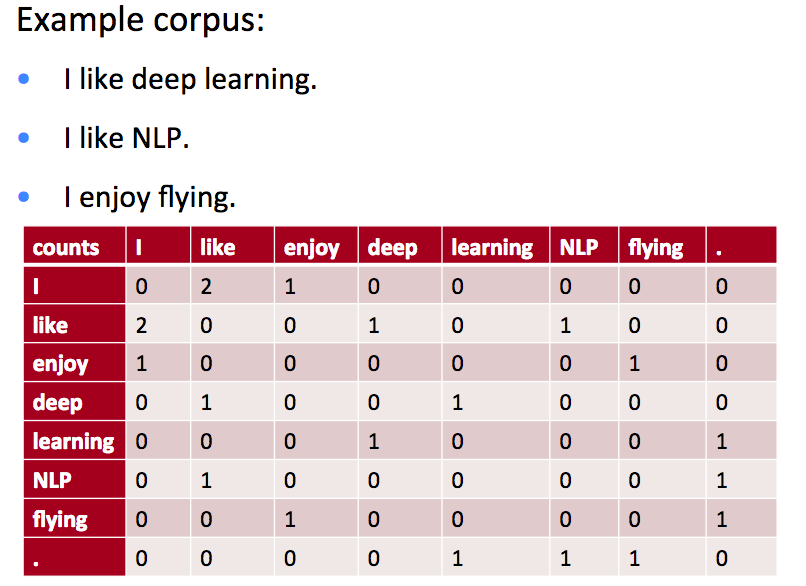
\includegraphics[scale=0.3]{pics/distributionalSocher.png}
\end{figure}


\footnotetext{Example taken from:    \url{http://cs224d.stanford.edu/lectures/CS224d-Lecture2.pdf}}
%\footnote{Source: \url{http://cs224d.stanford.edu/lectures/CS224d-Lecture2.pdf}}

\end{frame}



\begin{frame}{Word-context Matrices}
\begin{scriptsize}
The associations between words and contexts can be calculated using different approaches:
\begin{enumerate}
 \item Co-occurrence counts.
\item Positive point-wise mutual information (PPMI).
\item The significance values of a paired t-test.  
\end{enumerate}

The most common of those according to \cite{JurafskyBook} is PPMI.

Distributional methods are also referred to as count-based methods.

\end{scriptsize}
\end{frame}



\begin{frame}{PPMI}
\begin{scriptsize}
\begin{itemize}
\item  PMI calculates the log of the probability of word-context pairs occurring together over the probability of them being independent. 

\begin{equation}
 \operatorname{PMI}(w, c)= \log_2 \left( \frac{P(w,c)}{P(w)P(c)} \right) = \log_{2} \left ( \frac{\operatorname{count}(w,c)\times |D|}{\operatorname{count}(w)\times \operatorname{count}(c)} \right ) 
\end{equation}






\item Negative PMI values suggest that the pair co-occurs less often than chance. 
\item These estimates are unreliable unless the counts are calculated from very large corpora \cite{JurafskyBook}.
\item  PPMI corrects this problem by replacing negative values by zero:

\begin{equation}
 \operatorname{PPMI}(w, c)= \operatorname{max}(0,\operatorname{PMI}(w, c))
\end{equation}

\end{itemize}
\end{scriptsize}
\end{frame}



\begin{frame}{Distributed Vectors or Word embeddings}
\begin{scriptsize}
\begin{itemize}

\item Count-based distributional vectors increase in size with vocabulary i.e., can have a very high dimensionality.

\item Explicitly storing the co-occurrence matrix can be memory-intensive. 

\item Some classification models don't scale well to high-dimensional data.

\item  The neural network community prefers using \textbf{distributed representations}\footnote{Idea: The meaning of the word is ``distributed'' over a combination of dimensions.} or \textbf{word embeddings}.

\item  Word \textbf{embeddings} are low-dimensional continuous dense word vectors trained from document corpora using \textbf{neural networks}.

\item The dimensions are not directly interpretable i.e., represent latent features of  the  word,  ``hopefully capturing useful syntactic and semantic properties''~\cite{turian2010word}.

\item They have become a crucial component of neural network architectures for NLP.


\end{itemize}
\end{scriptsize}
\end{frame}






\begin{frame}{Distributed Vectors or Word embeddings (2)}
\begin{scriptsize}
\begin{itemize}

\item There are two main approaches for obtaining word embeddings:

\begin{enumerate}
\begin{scriptsize}

\item Embedding layers: using an embedding layer in a task-specific neural network architecture trained from labeled examples (e.g., sentiment analysis).

\item Pre-trained word embeddings: creating an auxiliary predictive task from unlabeled copora (e.g., predict the following word) in which word embeddings will naturally arise from the neural-network architecture.
\end{scriptsize}
\end{enumerate}


\item These approaches can also be combined: one can initialize an embedding layer of a task-specific neural network with pre-trained word embeddings obtained with the second approach.

\end{itemize}
\end{scriptsize}
\end{frame}


\begin{frame}{Distributed Vectors or Word embeddings (2)}
\begin{scriptsize}
\begin{itemize}


\item Most popular models based on the second approach are skip-gram \cite{Mikolov2013}, continuos bag-of-words \cite{Mikolov2013}, and Glove \cite{penningtonSM14}.

\item Word embeddings have shown to be more powerful than distributional approaches in many NLP tasks~\cite{baroni2014don}.

\item In \cite{amir2015SemEval}, they were used as \textbf{features} in a regression model for determining the association between Twitter words and \textbf{positive sentiment}. 

\end{itemize}
\end{scriptsize}
\end{frame}




\begin{frame}{Word2Vec}
\begin{scriptsize}
\begin{itemize}
\item Word2Vec is a software package that implements two neural network architectures for training word embeddings:  Continuos Bag of Words (CBOW) and Skip-gram.
\item It implements two  optimization models: Negative Sampling and Hierarchical Softmax.
\item These models are shallow neural networks that are trained to predict the contexts of words.
\end{itemize}
\end{scriptsize}
\end{frame}


% Good Word2Vec tutorial
%http://mccormickml.com/2016/04/19/word2vec-tutorial-the-skip-gram-model/

\begin{frame}{Skip-gram Model}
\begin{scriptsize}
\begin{itemize}
\item A neural network with one ``projection'' or ``hidden'' layer is trained for predicting the words surrounding a center word, within a window  of size $k$ that is shifted along the input corpus. 
\item The center and surrounding $k$ words correspond to the input and output layers of the network.
\item Words are initially represented by 1-hot vectors: vectors of the size of the vocabulary ($|V|$) with zero values in all entries except for the corresponding word index that receives a value of 1. 
\end{itemize}
\end{scriptsize}

\end{frame}



\begin{frame}{Skip-gram Model}
\begin{scriptsize}
\begin{itemize}
\item The output layer combines the $k$ 1-hot vectors of the surrounding words. 
\item The hidden layer has a dimensionality $d$, which determines the size of the embeddings (normally $d \ll |V|$).
\end{itemize}
\end{scriptsize}
  \begin{figure}[h]
        	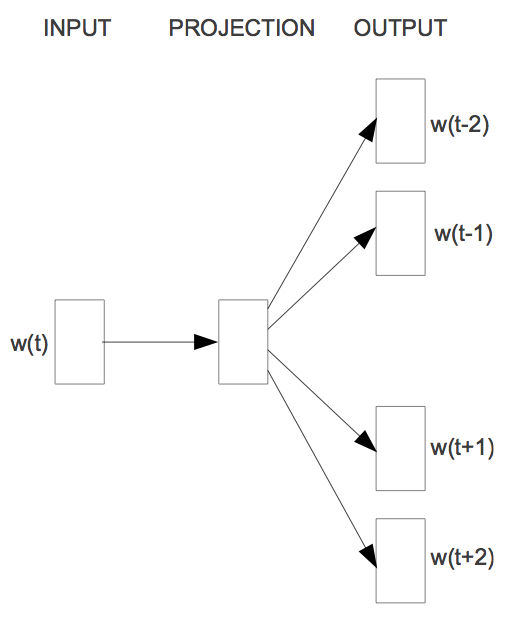
\includegraphics[scale = 0.4]{pics/skip-gram.png}
        \end{figure}

\end{frame}



\begin{frame}{Skip-gram Model}

  \begin{figure}[h]
        	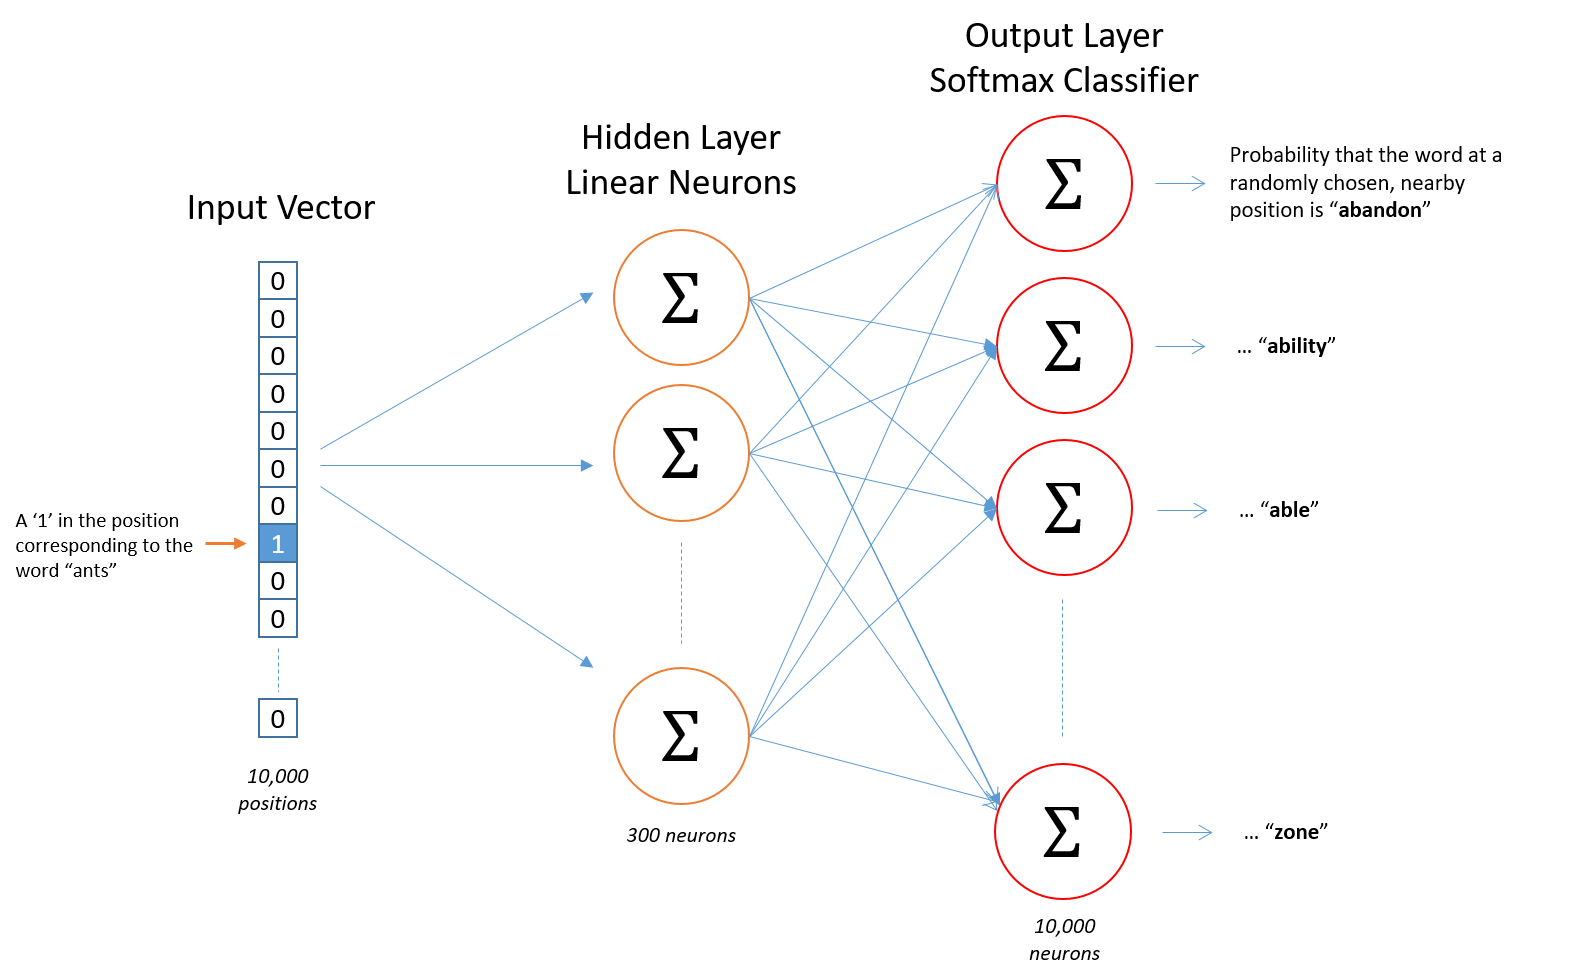
\includegraphics[scale = 0.4]{pics/skip_gram_net_arch.png}
        \end{figure}
\footnotetext{Picture taken from:    \url{http://mccormickml.com/2016/04/19/word2vec-tutorial-the-skip-gram-model/}}

\end{frame}


% we use hierarchical softmax where the vocabulary is represented as a Huffman binary tree. This follows previous observations that the frequency of words works well for obtaining classes in neural net language models [16]. Huffman trees assign short binary codes to frequent words, and this further reduces the number of output units that need to be evaluated


%If two different words have very similar “contexts” (that is, what words are likely to appear around them), then our model needs to output very similar results for these two words. And one way for the network to output similar context predictions for these two words is if the word vectors are similar. So, if two words have similar contexts, then our network is motivated to learn similar word vectors for these two words! Ta da!

%And what does it mean for two words to have similar contexts? I think you could expect that synonyms like “intelligent” and “smart” would have very similar contexts. Or that words that are related, like “engine” and “transmission”, would probably have similar contexts as well.

%This can also handle stemming for you – the network will likely learn similar word vectors for the words “ant” and “ants” because these should have similar contexts.

%https://arxiv.org/pdf/1402.3722.pdf

\begin{frame}{Parametrization of the Skip-gram model}
\begin{scriptsize}
\begin{itemize}

\item  We are given an input corpus formed by a sequence of  words $w_1, w_2, w_3, . . . , w_T$ and a window size $k$.

\item We denote target or (center) words by letter $w$ and surrounding context words by letter $c$.

\item The objective of the Skip-gram model is to maximize the average log probability of the context words given the target words:

\begin{displaymath}
 \frac{1}{T} \sum_{t=1}^T \sum_{c \in c_{1:k}}  \log p(c|w_t)
\end{displaymath}


\item The conditional probability of a context word $c$ given a center word $w$ is modeled with a softmax ($C$ is the set of all context words, which is usually the same as the vocabulary):


\begin{displaymath}
p(c|w) = \frac{e^{\vec{c}\cdot \vec{w}}}{ \sum_{c'\in C} e^{\vec{c}'\cdot \vec{w}}}
\end{displaymath}

\item Model's parameters $\theta$: $\vec{c}$ and $\vec{w}$ (vector representations of contexts and target words).

\end{itemize}
\end{scriptsize}
\end{frame}






\begin{frame}{Parametrization of the Skip-gram model}
\begin{scriptsize}
\begin{itemize}

\item Let $D$ be the set of correct word-context pairs (i.e., word pairs that are observed in the Corpus).

\item The optimization goal is to maximize the conditional likelihood of the contexts $c$:


\begin{equation}
\begin{split}
\operatorname{arg} \max_{\vec{c}, \vec{w}} & \quad \sum_{(w,c) \in D}{\log p(c|w)} = \sum_{(w,c) \in D} ( \log e^{\vec{c}\cdot \vec{w}} - \log \sum_{c'\in C} e^{\vec{c}'\cdot \vec{w}}  )
\end{split}
\end{equation}


\item Assumption: maximizing this function will result in good embeddings $\vec{w}$ i.e.,  similar words will have similar vectors.

\item The term $p(c|w)$ is computationally expensive because of the summation $\sum_{c'\in C} e^{\vec{c}'\cdot \vec{w}}$ over all the contexts $c'$.

\item Fix: replace the softmax with a hierarchical softmax (the vocabulary is represented with a Huffman binary tree). 

\item Huffman trees assign short binary codes to frequent words, reducing the number of output units to be evaluated.

\end{itemize}
\end{scriptsize}
\end{frame}



%The distributional hypothesis states that words in similar contexts have similar meanings. The objective above clearly tries to increase the quantity  for good word-context pairs, and decrease it for bad ones.  Intuitively, this means that words that share many contexts will be similar to each other (notealso that contexts sharing many words will also be similar to each other). This is, however, very hand-wavy.

% https://arxiv.org/pdf/1402.3722.pdf  Skip-gram and Negative Sampling are not the same

\begin{frame}{Skip-gram with Negative Sampling}
\begin{scriptsize}
\begin{itemize}

\item Negative-sampling (NS) is presented as a more efficient model for calculating skip-gram embeddings. 
\item However, it optimizes a different objective function \cite{goldberg2014word2vec}.


\item NS maximizes the probability that a word-context pair $(w, c)$ came from the set of correct word-context pairs $D$ using a sigmoid function:

\begin{displaymath}
P(D = 1| w,c_i) = \frac{1}{1+e^{-\vec{w} \cdot \vec{c_{i}}}}
\end{displaymath}

\item Assumption: the contexts words $c_i$ are independent from each other:

\begin{displaymath}
P(D = 1| w,c_{1:k}) = \prod_{i=1}^{k}{P(D = 1| w,c_i)} = \prod_{i=1}^{k}{\frac{1}{1+e^{-\vec{w} \cdot \vec{c_{i}}}}} 
\end{displaymath}

\item This leads to the following target function (log-likelihood): 

\begin{equation}
\begin{split}
\operatorname{arg} \max_{\vec{c}, \vec{w}} & \quad \log P(D = 1| w,c_{1:k}) = \sum_{i=1}^{k}{\log \frac{1}{1+e^{-\vec{w} \cdot \vec{c_{i}}}}}
\end{split}
\end{equation}





\end{itemize}
\end{scriptsize}
\end{frame}


\begin{frame}{Skip-gram with Negative Sampling (2)}
\begin{scriptsize}
\begin{itemize}


\item This objective has a trivial solution if we set $\vec{w}$,$\vec{c}$ such that $p(D=1|w,c)=1$ for every pair $(w,c)$ from $D$.
\item This is achieved by setting $\vec{w}=\vec{c}$  and $\vec{w} \cdot \vec{c} = K$ for all $\vec{w},\vec{c}$, where $K$ is a large number.
\item We need a mechanism that prevents all the vectors from having the same value, by disallowing some $(w, c)$ combinations. 
\item One way to do so, is to present the model with some $(w, c)$ pairs for which $p(D= 1|w, c)$ must be low, i.e.
pairs which are not in the data.  
\item This is achieved sampling negative samples from $\tilde{D}$. 





\end{itemize}
\end{scriptsize}
\end{frame}


\begin{frame}{Skip-gram with Negative Sampling (3)}
\begin{scriptsize}
\begin{itemize}

\item Sample $m$ words for each word-context pair  $(w,c) \in D$.
\item Add each sampled word $w_i$ together with the original context $c$ as a negative example to $\tilde{D}$.

%\item $\tilde{D}$ being $m$ times larger than $D$. 

%\item The number of negative samples $m$ is a parameter of the algorithm.

\item Final objective function:
\begin{equation}
\begin{split}
\operatorname{arg} \max_{\vec{c}, \vec{w}} & \quad \sum_{(w,c) \in D}{\log P(D = 1| w,c_{1:k})} + \sum_{(w,c) \in \tilde{D}} \log P(D = 0| w,c_{1:k})
\end{split}
\end{equation}

\item The negative words are sampled from smoothed version of the corpus frequencies:
\begin{displaymath}
\frac{\#(w)^{0.75}}{\sum_{w'}\#(w')^{0.75}}
\end{displaymath}

\item This gives more relative weight to less frequent words.

\end{itemize}
\end{scriptsize}
\end{frame}






\begin{frame}{Continuos Bag of Words: CBOW}
\begin{scriptsize}
\begin{itemize}
\item  Similar to the skip-gram model but now the center word is predicted from the surrounding context.
 \begin{figure}[h]
    	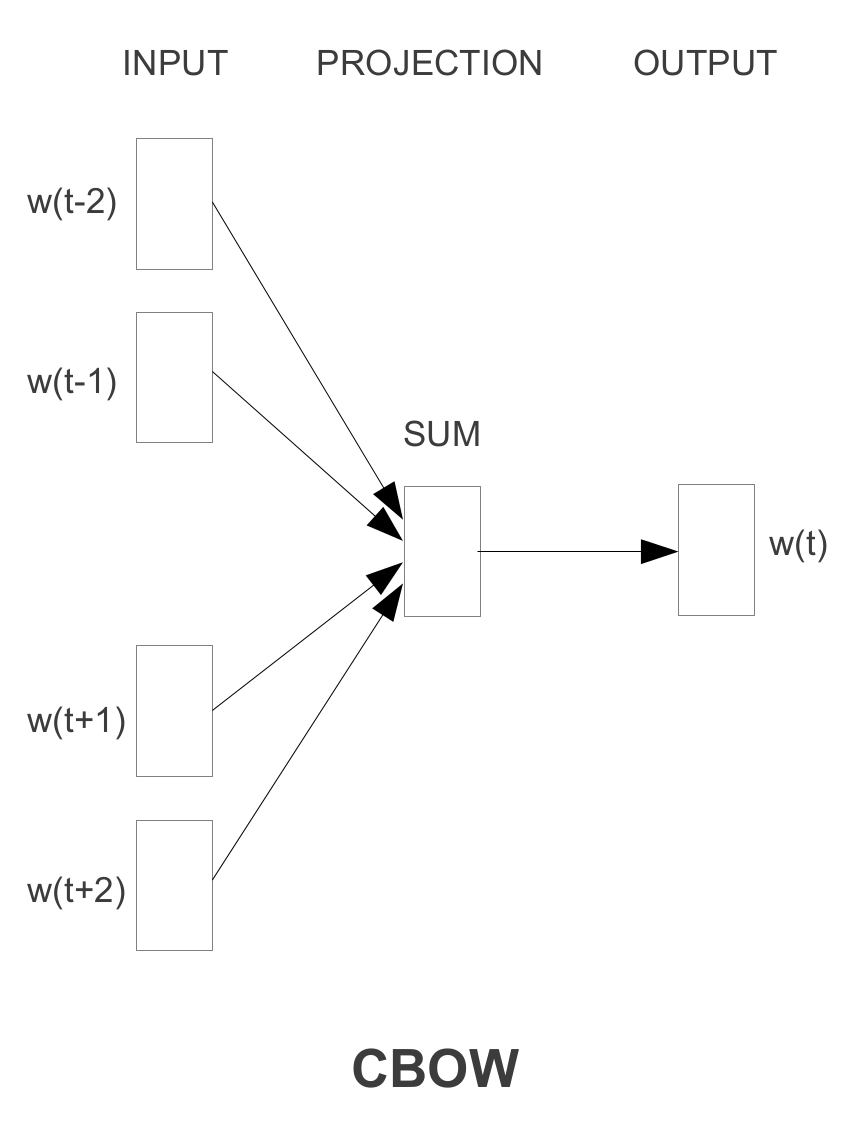
\includegraphics[scale = 0.55]{pics/CBOW.png}
    \end{figure}
       
        
\end{itemize}
\end{scriptsize}
\end{frame}



\begin{frame}{GloVe}
\begin{scriptsize}
\begin{itemize}
\item  GloVe (from global vectors) is another popular method for training word embeddings \cite{penningtonSM14}.

\item It constructs an explicit word-context
matrix, and trains the word and context vectors $\vec{w}$ and $\vec{c}$ attempting to satisfy:

\begin{equation}
\vec{w} \cdot \vec{c} + b_{[w]}+b_{[c]} = \log \#(w,c) \quad \forall (w,c) \in D
\end{equation}

\item where $b_{[w]}$ and $b_{[c]}$ are word-specific and context-specific trained biases.

        
\end{itemize}
\end{scriptsize}
\end{frame}



\begin{frame}{GloVe (2)}
\begin{scriptsize}
\begin{itemize}

\item In terms of matrix factorization, if we fix $b_{[w]}=\log \#(w)$ and $b_{[c]}=\log \#(c)$ we'll get an objective that is very similar to factorizing the word-context PMI matrix, shifted by $\log (|D|)$.
\item In GloVe the bias parameters are learned and not fixed, giving it another degree of freedom.

\item The optimization objective is weighted least-squares loss, assigning more weight to the correct reconstruction of frequent items.
       
\item When using the same word and context vocabularies, the model suggests representing each word as the sum of its corresponding word and context embedding vectors.   
        
\end{itemize}
\end{scriptsize}
\end{frame}


\begin{frame}{Word Analogies}
\begin{scriptsize}
\begin{itemize}
   
\item Word embeddings can capture certain semantic relationships, e.g. male-female, verb tense and country-capital relationships between words.

\item For example, the following relationship is found for word embeddings
trained using Word2Vec: $\vec{w}_{king} - \vec{w}_{man} + \vec{w}_{woman} \approx \vec{w}_{queen}$.

    
\end{itemize}

 \begin{figure}[h]
    	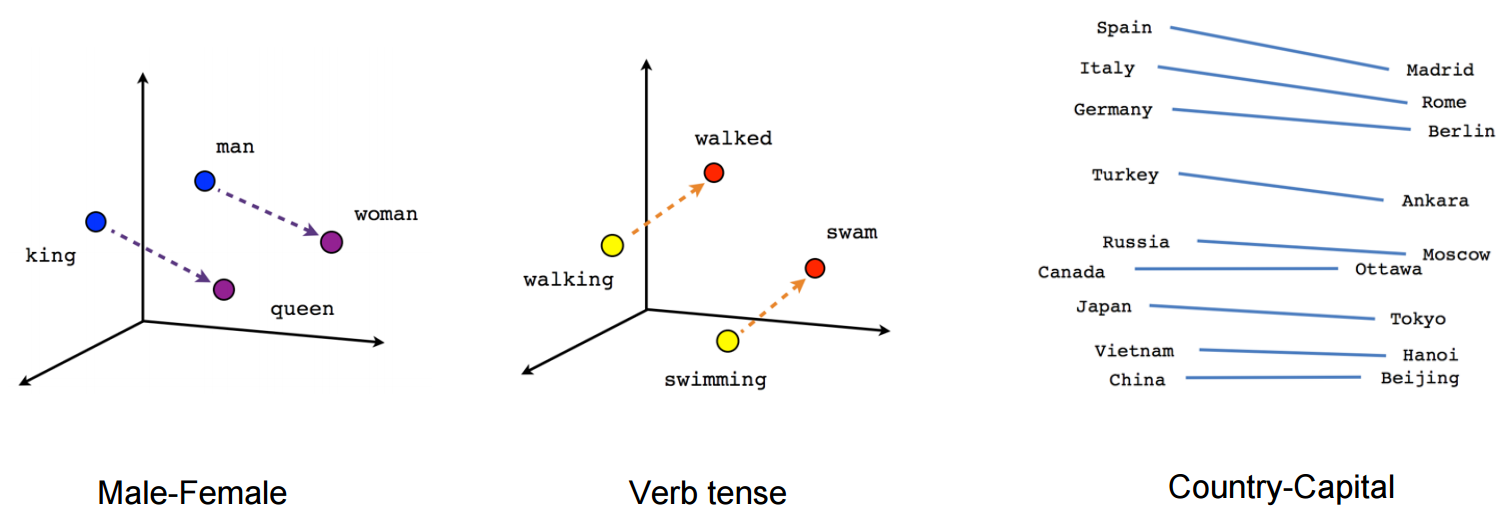
\includegraphics[scale = 0.2]{pics/linear-relationships.png}
    \end{figure}
\footnotemark{Source: \url{https://www.tensorflow.org/tutorials/word2vec}}

\end{scriptsize}
\end{frame}



\begin{frame}{Correspondence between Distributed and Distributional Models}
\begin{scriptsize}
\begin{itemize}
       
\item Both the distributional ``count-based'' methods and the distributed ``neural'' ones are based on the distributional hypothesis.

\item The both attempt to capture the similarity between words based on the similarity between the contexts in which they occur.      
       
\item Levy and Goldebrg showed in \cite{levy2014neural} that Skip-gram negative sampling (SGNS) is implicitly factorizing a word-context matrix, whose cells are the pointwise mutual information (PMI) of the respective word and context pairs, shifted by a global constant. 

%https://levyomer.files.wordpress.com/2014/09/neural-word-embeddings-as-implicit-matrix-factorization.pdf

\item This ties the neural methods and the traditional ``count-based'' suggesting that in a deep sense
the two algorithmic families are equivalent.
     
\end{itemize}
\end{scriptsize}
\end{frame}


\begin{frame}{FastText}
\begin{scriptsize}
\begin{itemize}
  
\item FastText embeedings extend the skipgram model to take into account the internal structure of words while learning word representations \cite{bojanowski2016enriching}.

\item A vector representation is associated with each character $n$-gram.

\item  Words are represented as the sum of these representations. 

\item Taking the word \emph{where} and $n = 3$, it will be represented by the character $n$-grams: $<$wh, whe, her, ere, re$>$, and the special sequence $<$where$>$.

\item Note that the sequence \emph{$<$her$>$}, corresponding to the word ``her'' is different from the tri-gram ``her'' form the word ``here''. 

\item FastText is useful for morphologically rich languages. For example, the words ``amazing'' and ``amazingly'' share information in FastText through their shared $n$-grams, whereas in Word2Vec these two words are completely unrelated.    
   
\end{itemize}
\end{scriptsize}
\end{frame}


\begin{frame}{FastText (2)}
\begin{scriptsize}
\begin{itemize}
  
\item Let $\mathcal{G}_{w}$ be the set of $n$-grams appearing in $w$.

\item FastText associates a vector $\vec{g}$ with each $n$-gram in $\mathcal{G}_{w}$.

\item In FastText the probability that  a word-context pair $(w, c)$ came from the input corpus $D$ is calculated as follows:

\begin{displaymath}
 P(D | w, c) = \frac{1}{1+e^{-s(w,c)}}
\end{displaymath}

where,

\begin{displaymath}
s(w,c) = \sum_{g \in {G}_{w}} \vec{g} \cdot \vec{c}.
\end{displaymath}

\item The negative sampling algorithm can be calculated in the same form as in the skip-gram model with this formulation.

\end{itemize}
\end{scriptsize}
\end{frame}





\begin{frame}{Sentiment-Specific Phrase Embeddings}
%https://pdfs.semanticscholar.org/107f/b80ff801894b6191d0613af41aba91c134a4.pdf
\begin{scriptsize}
\begin{itemize}
\item Problem of word embeddings: antonyms can be used in similar contexts e.g., my car is nice vs my car is ugly.

\item In \cite{TangCol14}  \textbf{sentiment-specific} word embeddings are proposed  by combining the skip-gram model with emoticon-annotated tweets :) :( .

\item These embeddings are used for \textbf{training} a word-level polarity classifier.

\item The model integrates sentiment information into the continuous representation of phrases by developing a tailored neural architecture.

\item Input: $\{w_i,s_j,pol_j\}$, where $w_i$ is a phrase (or word), $s_j$ the sentence, and $pol_j$ the sentence's polarity.

\end{itemize}
\end{scriptsize}
\end{frame}


\begin{frame}{Sentiment-Specific Phrase Embeddings (2)}
%https://pdfs.semanticscholar.org/107f/b80ff801894b6191d0613af41aba91c134a4.pdf
\begin{scriptsize}
\begin{itemize}

\item The training objective uses the embedding of $w_i$ to predict its context words (in the same way as the skip-gram model), and uses the sentence representation $se_j$ to predict $pol_j$.


\item Sentences ($se_j$) are represented by averaging the word vectors of their words.

\item The  objective of the sentiment part is to maximize the average of log sentiment probability: 
\begin{displaymath}
f_{sentiment}= \frac{1}{S}\sum_{j=1}^{S}\log p(pol_j|se_j)
\end{displaymath}

\item The final training objective is to maximize the linear combination of the skip-gram and sentiment objectives: 
\begin{displaymath}
f = \alpha f_{skipgram} + (1- \alpha)f_{sentiment}
\end{displaymath}

\end{itemize}
\end{scriptsize}
\end{frame}



\begin{frame}{Sentiment-Specific Phrase Embeddings}
%https://pdfs.semanticscholar.org/107f/b80ff801894b6191d0613af41aba91c134a4.pdf


  \begin{figure}[h]
        	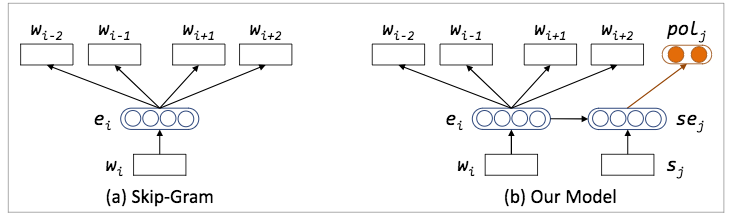
\includegraphics[scale = 0.4]{pics/SSPE.png}
        \end{figure}

  \begin{figure}[h]
        	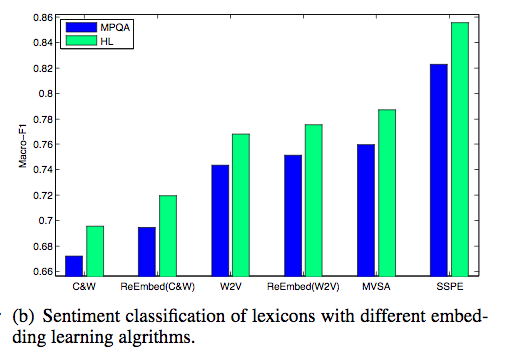
\includegraphics[scale = 0.3]{pics/SSPERes.png}
        \end{figure}


\end{frame}






\begin{frame}{Gensim}
\begin{scriptsize}
Gensim is an open source Python library for natural language processing that implements many algorithms for training word embeddings.


\begin{itemize}
 \item \url{https://radimrehurek.com/gensim/}

  \item \url{https://machinelearningmastery.com/develop-word-embeddings-python-gensim/}
 
\end{itemize}



  \begin{figure}[h]
        	
\includegraphics[scale = 0.3]{pics/gensim.png}
        \end{figure}



\end{scriptsize}
\end{frame}







\begin{frame}
\frametitle{Questions?}
%\vspace{1.5cm}
\begin{center}\LARGE Thanks for your Attention!\\ \end{center}



\end{frame}

\begin{frame}[allowframebreaks]\scriptsize
\frametitle{References}
\bibliography{bio}
\bibliographystyle{apalike}
%\bibliographystyle{flexbib}
\end{frame}  


%%%%%%%%%%%%%%%%%%%%%%%%%%%

\end{document}
